\documentclass[10pt]{article}
\usepackage[margin=0.7in]{geometry}
\usepackage{amsmath,amssymb,graphicx,hyperref,array}
\setlength{\parindent}{0pt}
\setlength{\parskip}{6pt}
\setlength{\emergencystretch}{2em}
\hypersetup{colorlinks=true,urlcolor=blue}
\begin{document}
{\Large\bfseries J2: squared negation-translation witness}\par
\texttt{TASK-20261031-8a54e2}; joint \texttt{J2\_commutator\_witness}.\par
Producer PR \#2417: \texttt{f4330e1a29feb8fdea9f1eab7131ae5cde2e2b6f}.\\
Plan PR \#2847: \texttt{774a6a86f181740285ed9834a648b40fb9aa8ece}.

The companion witness has augmentation $-1$ and affine group-algebra image $0$, including $B=1,n=2$. Its source-declared statements faithfully express that result. Exact finite controls passed. Fresh Lean replay was not allocated to this reviewer, so the formal-review outcome remains \textbf{inconclusive}; the source-fidelity finding is \textbf{faithful scoped}.

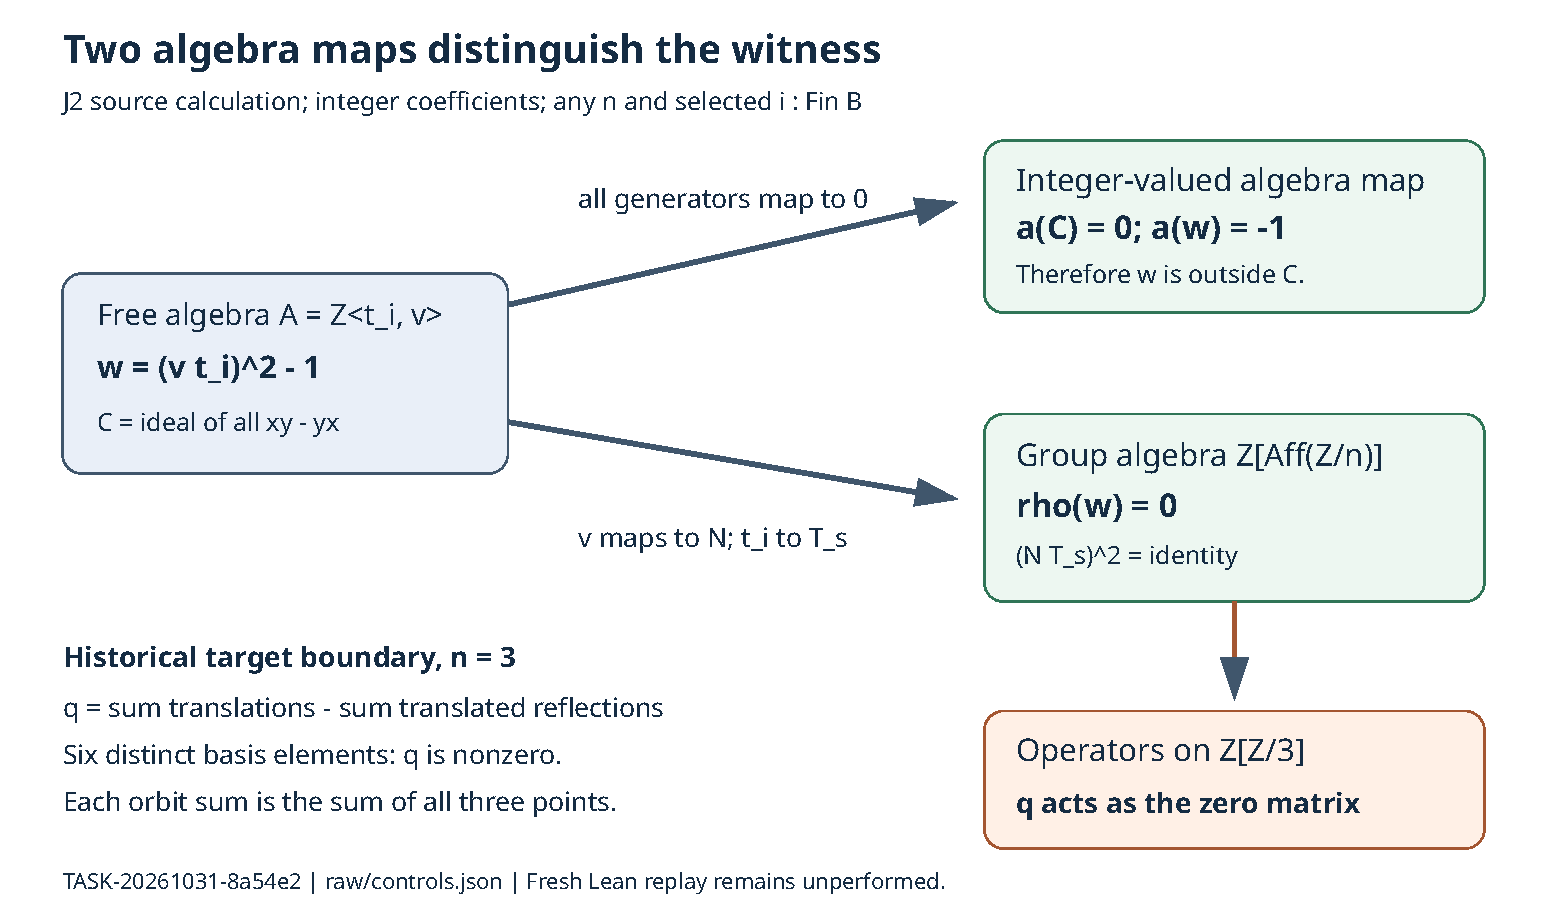
\includegraphics[width=\linewidth]{diagram.pdf}

\textbf{Exact declarations.} In namespace \texttt{CryptoResearch.NCP}:
\begin{quote}\small\ttfamily
neg\_translate\_square\_not\_in\_commutators\\
neg\_translate\_square\_in\_action\_kernel
\end{quote}
These declarations concern the same element
$(\nu t_i)^2-1$. The first is universally quantified in $B$ and $i:\mathrm{Fin}\,B$; the second also in $n:\mathbb N$ and $s:\mathrm{Fin}\,B\to\mathrm{ZMod}\,n$.
The target is $\mathbb Z[\mathrm{affineGroup}(\mathrm{ZMod}\,n)]$, with the affine group a subgroup of actual permutations. No oddness, primality or surjectivity assumption occurs.

\textbf{Calculation.} The algebra map $a$ sending every free generator to zero kills every $xy-yx$ and hence the two-sided ideal $C$ they generate. But $a((\nu t_i)^2-1)=-1$. Under permutation composition, $NT_s(x)=-(x+s)$ and $(NT_s)^2(x)=x$. Extending to group-algebra basis elements therefore sends the witness to zero. At $n=2,s=1$, $N$ is identity, $T_s$ is the transposition, and its square is identity. At $B=0$ there is no selected $i$; the older $\nu^2-1$ witness still applies.

\newpage
{\large\bfseries Controls and the historical target boundary}

\textbf{Exact controls.} The standalone integer/permutation checker imports no producer code. It checks all translations for moduli $1,\ldots,5$: 15 cases and 55 point evaluations. All squared witnesses map to zero and have zero-generator augmentation $-1$. Removing the square fails at $n=2,s=1$. Sending generators to 1 also fails to separate the witness. At $n=3,s=1$, $\nu t-t\nu$ has a nonzero group-algebra image: the witness establishes $K\ne C$, not $C\subsetneq K$.

\textbf{The $n=2$ full-presentation control.} For the historical ideal $J$, the substitution $t\mapsto1,\nu\mapsto-1$ kills translation commutators, $\nu^2-1$, $(\nu t)^2-1$, and all lattice binomials. It maps $\nu-1$ to $-2$. But $\nu-1$ is in the action evaluation kernel when $n=2$. Thus the full historical equality does not extend to $n=2$. The exact producer note already states this boundary; the companion witness remains valid there.

\textbf{A separate historical bridge breaks at odd order.} For $G=\mathbb Z/3$, set
\[
q=(\delta_1+\delta_T+\delta_{T^2})-(\delta_N+\delta_{TN}+\delta_{T^2N}).
\]
Its six basis elements are distinct, so $q\ne0$ in the group algebra. Both sums send every basis point to the sum of all three points, so $q$ acts as zero on $\mathbb Z[G]$. The raw control records all six coefficients and the $3\times3$ zero matrix. A nonsingular realization is $E/\mathbb F_5:y^2=x^3+4x+2$, with affine points $(3,1),(3,4)$ and infinity, so $E(\mathbb F_5)=G$ has order 3. The control checks point enumeration and nonsingularity, not the elliptic-curve group law. Thus the historical note's group-algebra inclusion into point operators is false; a faithful permutation group action need not give an injective algebra representation.

\textbf{Additional obligations for full kernel equalities.} Define the free group and historical ideal $J$; prove the dihedral normal form and exact lattice kernel; prove all of $J$ maps to zero; prove the converse by a quotient basis or a justified finite-rank argument; supply sign faithfulness and generation hypotheses; bridge the cyclic model to the curve. A claim about point operators must instead use the actual representation map and account for its additional kernel.

\textbf{Verification limits and next action.} No Lean/Lake process, axiom audit, kernel rechecker, experiment or cloud job was launched. Parent dispatch retained heavy-build ownership elsewhere. Memory was not measured to be scarce. Exact-pin named-declaration replay, elaborated types, complete input manifests and transitive axiom checks remain to be supplied by an owned verifier. The historical embedding sentence requires a new producer revision separating the two target algebras. This packet changes no official scientific status.

\begin{flushleft}\small
\textbf{Sources and reproducibility.} See \texttt{../review.md} for the full source-linked report; \texttt{source\_manifest.json} binds every source by SHA-256 and revision. Producer sources are \texttt{CommutatorCompanion.lean}, \texttt{CommutatorIdeal.lean} and \texttt{THM\_COMMUTATOR\_KERNEL1.md}, retained under \texttt{inputs/}. The pinned mathlib primary sources for FreeAlgebra, TwoSidedIdeal.Kernel and permutation composition were inspected at \texttt{cfc55fc58714a59dc06e6e79edc6d1d95140d3c2}. Toolchain: Lean 4.35.0. Independent arithmetic output: \texttt{controls.json}; command and hashes: \texttt{controls\_receipt.json}. No sibling report was read. Sole archive owner: \texttt{TASK-20261031-20ed91}.
\end{flushleft}
\end{document}
